\documentclass[12pt]{article}

\usepackage{upgreek}

\usepackage{amsmath}

\usepackage{graphicx}
\graphicspath{ {imgs/} }

\usepackage{dsfont}

\usepackage{mathtools}

\usepackage{hyperref}

\usepackage[utf8]{inputenc}

\usepackage{mathtools}

\usepackage{textcomp}

\usepackage[english]{babel}

\usepackage{tikz}

\usepackage{tcolorbox}

\usepackage{amsthm,amssymb}

\setlength{\parindent}{0cm}

\renewcommand\qedsymbol{$\blacksquare$}

\usepackage{fancyhdr}
 
\pagestyle{fancy}
\fancyhf{}
\fancyhead[LE,RO]{Graph Theory -- Fall 2017}
\fancyhead[RE,LO]{Joshua Concon}
\fancyfoot[CE,CO]{\leftmark}
\fancyfoot[LE,RO]{\thepage}


\begin{document}

\title{MATC32: Graph Theory\\ Lecture Notes}
\date{University of Toronto Scarborough -- Fall 2017}
\author{Joshua Concon}
\maketitle
Pre-reqs are MATB24, which is the second course on linear algebra at UTSC.
Instructor is Dr. Louis de Thanhoffer de Volcsey. I highly recommend sitting at the front since he likes to teach with the board. If you find any problems in these notes, feel free to contact me at conconjoshua@gmail.com.

\tableofcontents

\pagebreak

\section{Tuesday, September 5, 2017}

\subsection{The Seven Bridges of Konigsberg}

So basically there's this city called Konigsberg where a river flows through, and because of that, there are 7 bridges in the city. The bridges look like this:\\
\\
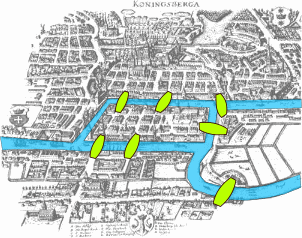
\includegraphics{Konigsberg_bridges}\\
\\

There problem that came up is whether or not it was possible to walk through every bridge in the city once in the same walk. This problem was eventually solved by Euler.\\
\\
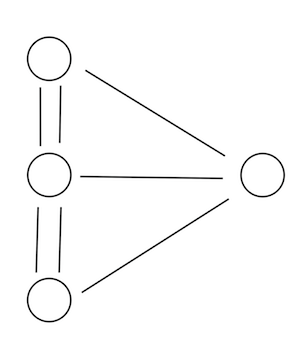
\includegraphics{Konigsberg_bridges_graph}\\
\\
It can be simplified to this. This is called a 'Graph', the circles are called 'nodes' or 'vertices' and the lines are called 'edges'. The different parts of the city are represented by the nodes and the bridges are represented by the edges.\\
\\
\begin{tcolorbox}[title=Definition: Graph ($G$)]
	\begin{enumerate}
		\item{Contains a set $V(G) =$ the set of nodes}
		\item{Contains a set $E(G) =$ the set of edges}
	\end{enumerate}
	A graph is called \textbf{Simple} if the graph has no loops and does not have multiple edges (i.e. Each edge is an unordered pair of distinct vertices).\\
	A graph is called a \textbf{Loop} if there is an edge that connects a vertex to itself.
\end{tcolorbox}

\begin{tcolorbox}[title=Definition: Path]
	A set of edges denoted by vertices $v_1, v_2, ..., v_n$ where there is a node between every edge between $v_i$ and $v_{i+1}$ $\forall i, 1 \leq i \leq n-1$
\end{tcolorbox}

\subsection{(Outline) Solution to Konigsberg}

Assume the graph has a path containing all edges $u_1,...,u_n$.\\
\\
Consider a vertex that isn't the first or last vertex travelled in the path (i.e. any vertex excluding $u_1$ and $u_n$).\\
\\
There must be an even number of edges for each of the nodes in between the edges in the path (excluding the first and the last node visited, unless the first and the last node visited are the same node).\\
\\
Since there are an odd number of adjacent nodes for all 4 nodes, this path does not exist. Therefore, there is no solution to Konigsberg.

\newpage

\section{Friday, September 8, 2017}

\subsection{Graphs}

\begin{tcolorbox}[title=Definition: Graphs]
	A graph $G$ consists of 2 (finite) sets:
	\begin{itemize}
		\item{$V(G)$ : vertex set}
		\item{$E(G)$ : edge set}
	\end{itemize}

	Together with an assignment from $E(G)$ to the set of subsets $V(G)$, where the subset is of size 1 or 2, containing the node(s) at the ends of the endpoints of each edge.
\end{tcolorbox}

If an edge has the same node at both of it's endpoints, it is called a \textbf{loop}.\\
\\
If 2 vertices are endpoints of more than one edge, we say that they are \textbf{multiply-edged}.\\
\\
A graph without multiply-edged vertices is called \textbf{simple}.\\
\\
\underline{Example:}

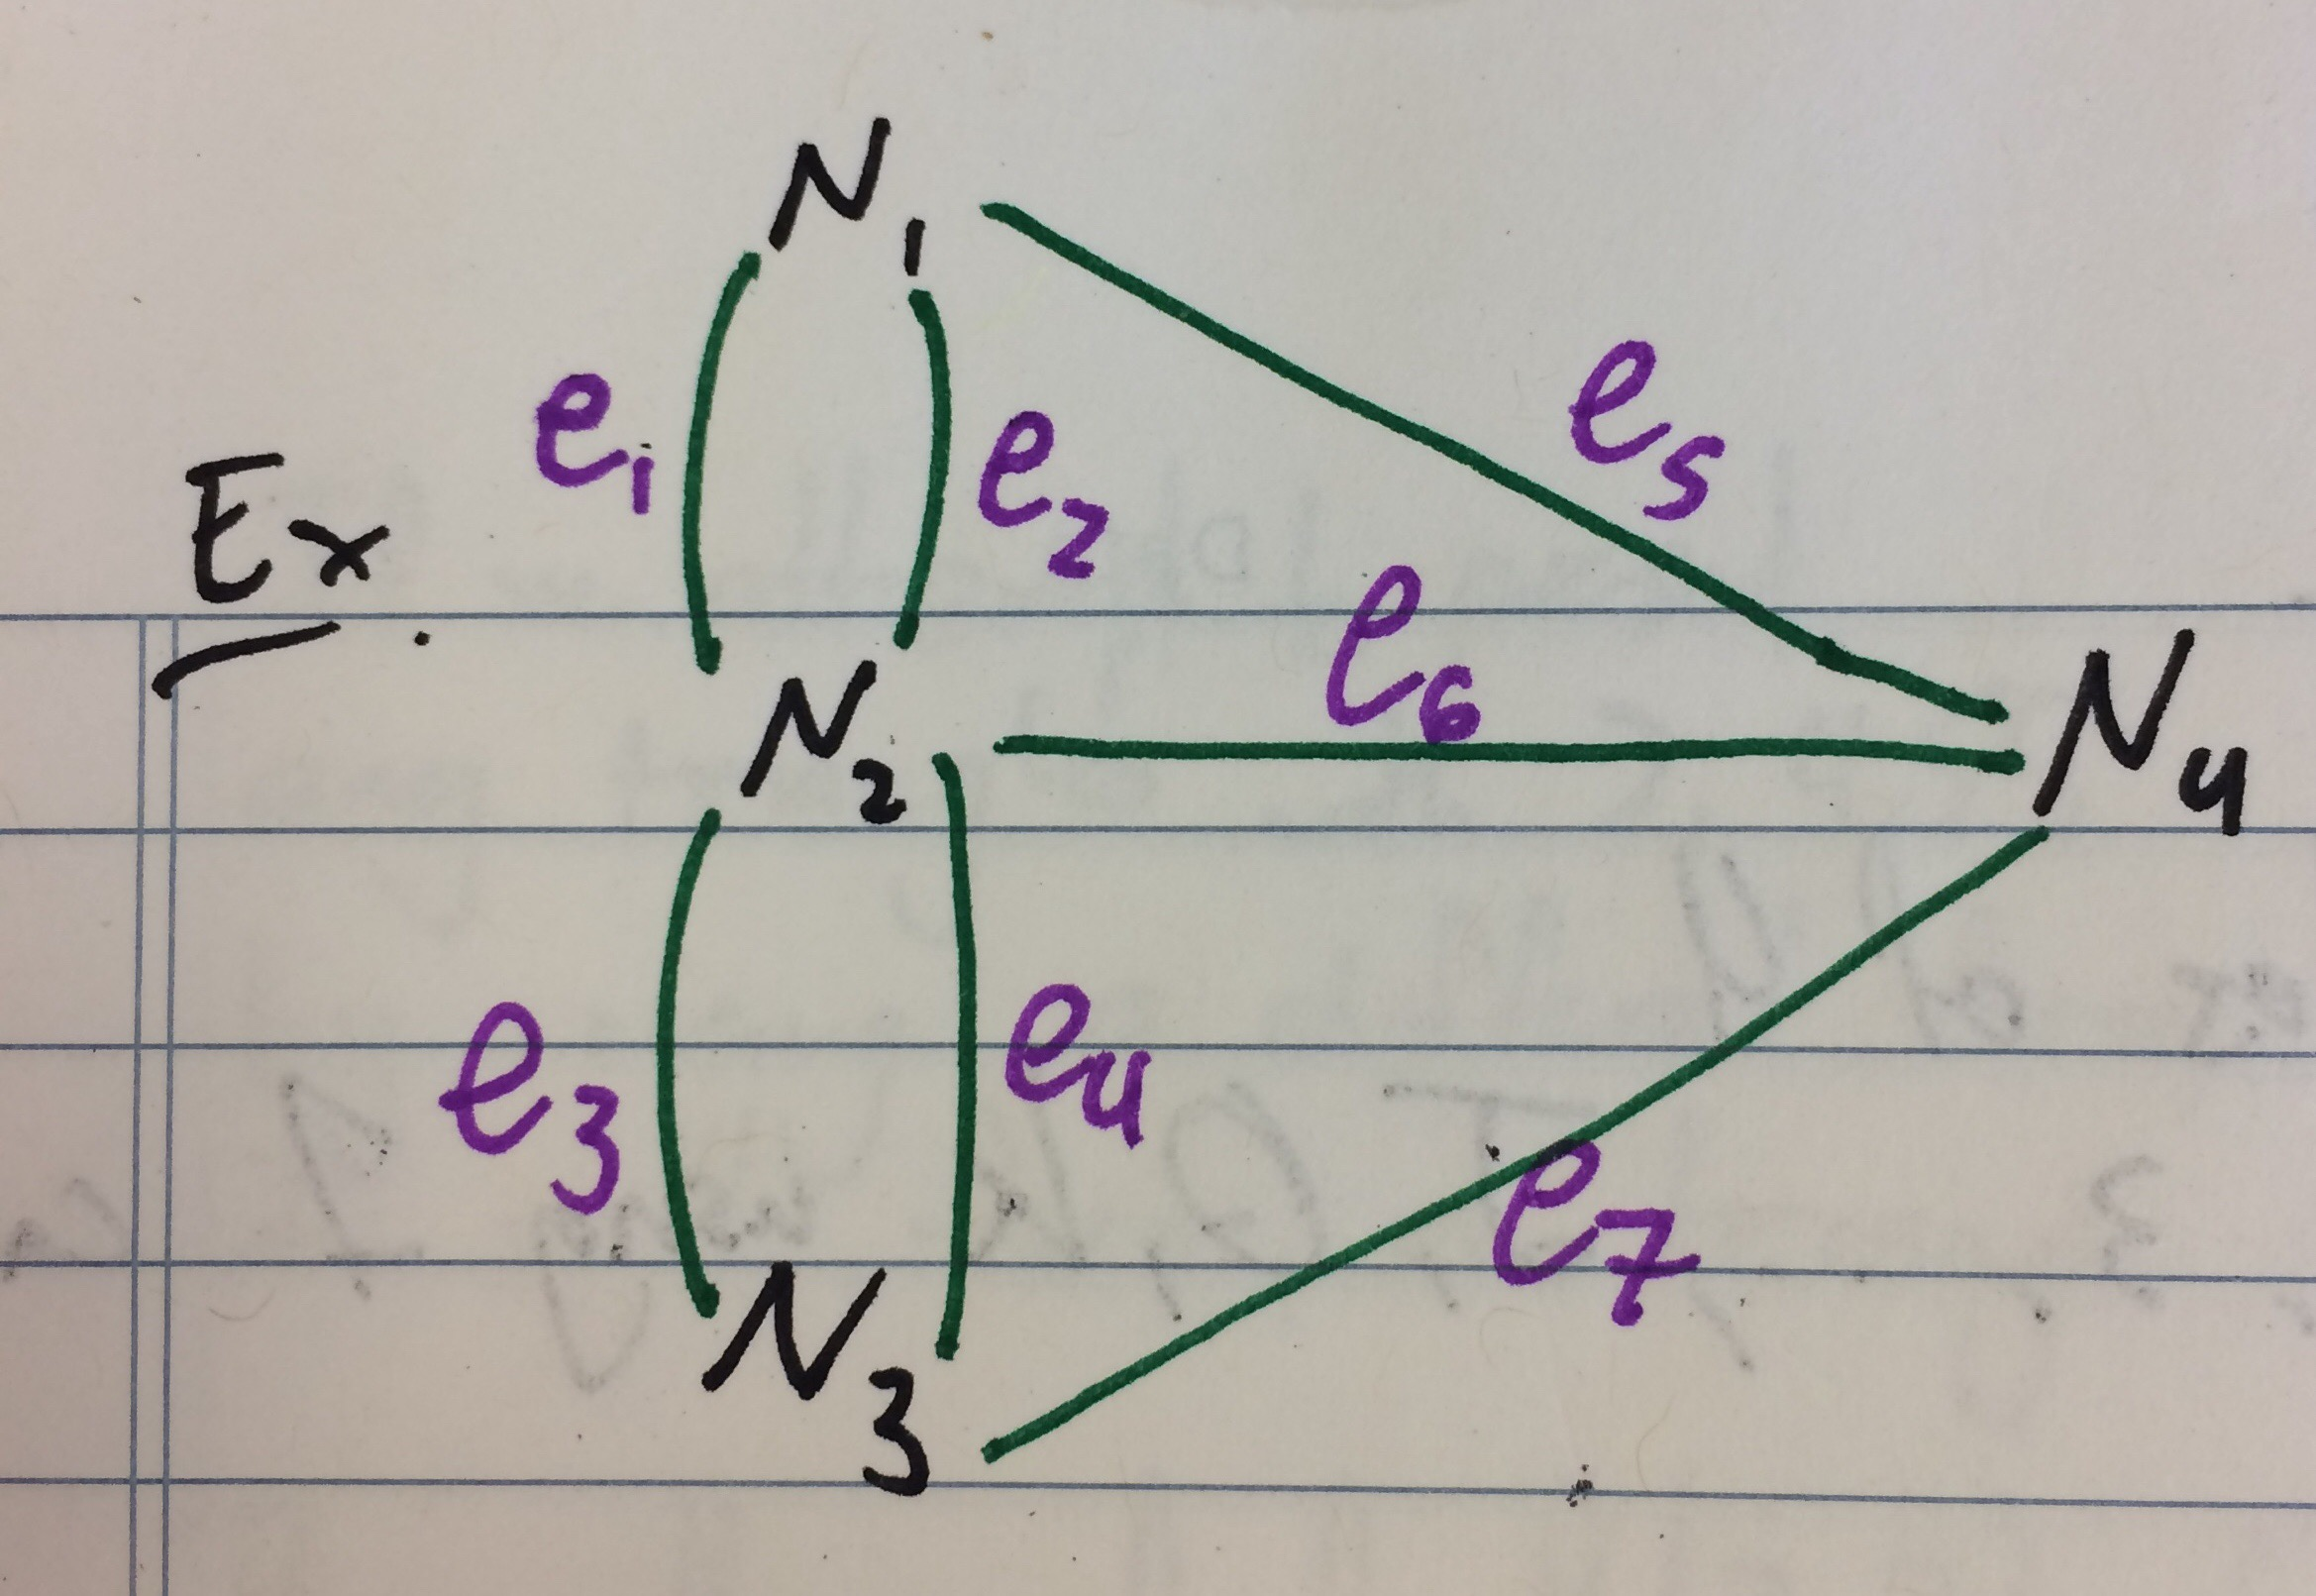
\includegraphics[scale=0.125]{lec2-1}

$$E(G) = \{ e_1, ... , e_7 \}$$
$$V(G) = \{ N_1, ... , N_4 \}$$

some of the assignments of $E(G) \mapsto V(G)$ include:
$$e_5 \mapsto \{ N_1, N_4 \}$$

\textbf{Adjacent edges} are edges with a vertex that is a common endpoint.

\subsection{Graph Theory Applications}

\subsubsection{Uber}

$$V = \text{People Using Uber (both drivers and passengers)}$$
$$E = \text{If it is realistic for a driver to pick up a person}$$

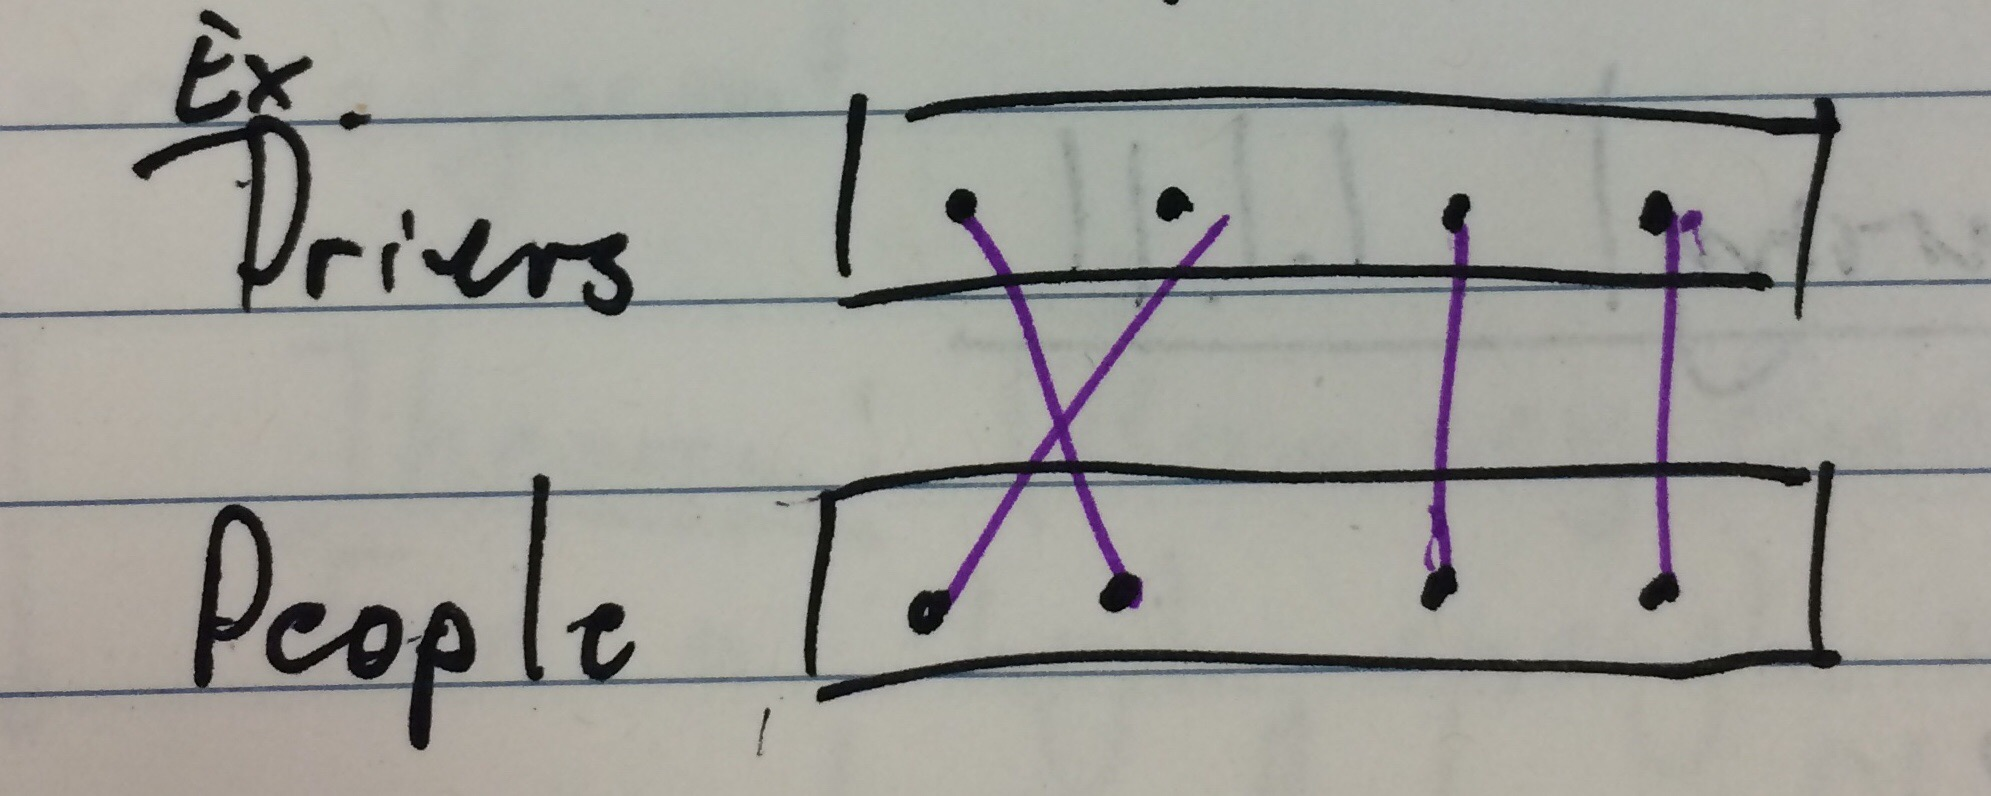
\includegraphics[scale=0.125]{lec2-2}

\begin{tcolorbox}[title=Definition: Matching]
	A \textbf{matching} in a group is a set of edges, none of which are adjacent
\end{tcolorbox}

\underline{Note:} $V(G) = S_1 \sqcup S_2$ and there are no edges between of $S_1$ with respect to $S_2$ ($\sqcup$ : refers to a union between two disjoint sets).\\
\\
These two sets $S_1, S_2$ are independent sets\\
\\
A \textbf{bipartite} graph has $V(G) = S_1 \sqcup S_2$ where both $S_1, S_2$ are independent.

\subsubsection{Monge's Theorem (on matching)}

Split a deck of 52 cards into 13 piles of 4, is it always possible to count an ace,2,3,...., Jack, Queen, King using 1 card drawn from each pile?

\subsubsection{Marriage (Stable) Problem}

Matching $n$ men with $n$ women

\subsubsection{Scheduling (Graph Colouring)}

Let $V$ represent different courses, and edges between courses mean that a student can take both courses at the same time. The problem is to reduce the edges between vertices with the same label or colour.\\
\\
$X(G)$ is the chromatic number of a graph $G$ and is the minimum number of colours needed to colour a graph without the edges having endpoints with two vertices of the same colour. To distribute these colours, there is a mapping from $V(G) \mapsto C$ where $C$ is a set of colours.\\
\\
\underline{Statement:} In a room of people, we can always be certain that 3 people either know each other or are all strangers for a room of 6+ people. So if we represent the people in the room as vertices in a non simple graph, and edge connections between people as the two unique people at the endpoints refer to familiarity or unfamiliarity, then you can always form a triangle with the edges.\\
\\
This is the proof of $R(3,3)=6$ for Ramsey's Theorem.\\
\\
\begin{tcolorbox}[title=Definition: Complete Graph]
	A Complete Graph is a simple graph where any 2 vertices are adjacent.
\end{tcolorbox}

A \textbf{clique} is a subset of vertices $C$ such that all vertices are adjacent.

\begin{tcolorbox}[title=Theorem: Ramsey's theorem]
	For a high enough number $R(n,m)$, we can guarantee that after colouring a complete graph of $m$ vertices with $2$ colours (in any way), there will be a clique of $n$ vertices of the same colour.
\end{tcolorbox}

\subsubsection{Network Problems}

A path is a series of vertices $v_1, .., v_n$ where $v_i$ and $v_{i+1}$ are adjacent for all $i, 1 \leq i \leq n-1$.\\
\\
Say 2 vertices are \textbf{connected} if there exists a path between them.\\
\\
Cutting number of 2 vertices $m,n$ are the amount of vertices that need to be removed such that vertices $m,n$ are not connected.
\\
\\
\underline{Example:}\\
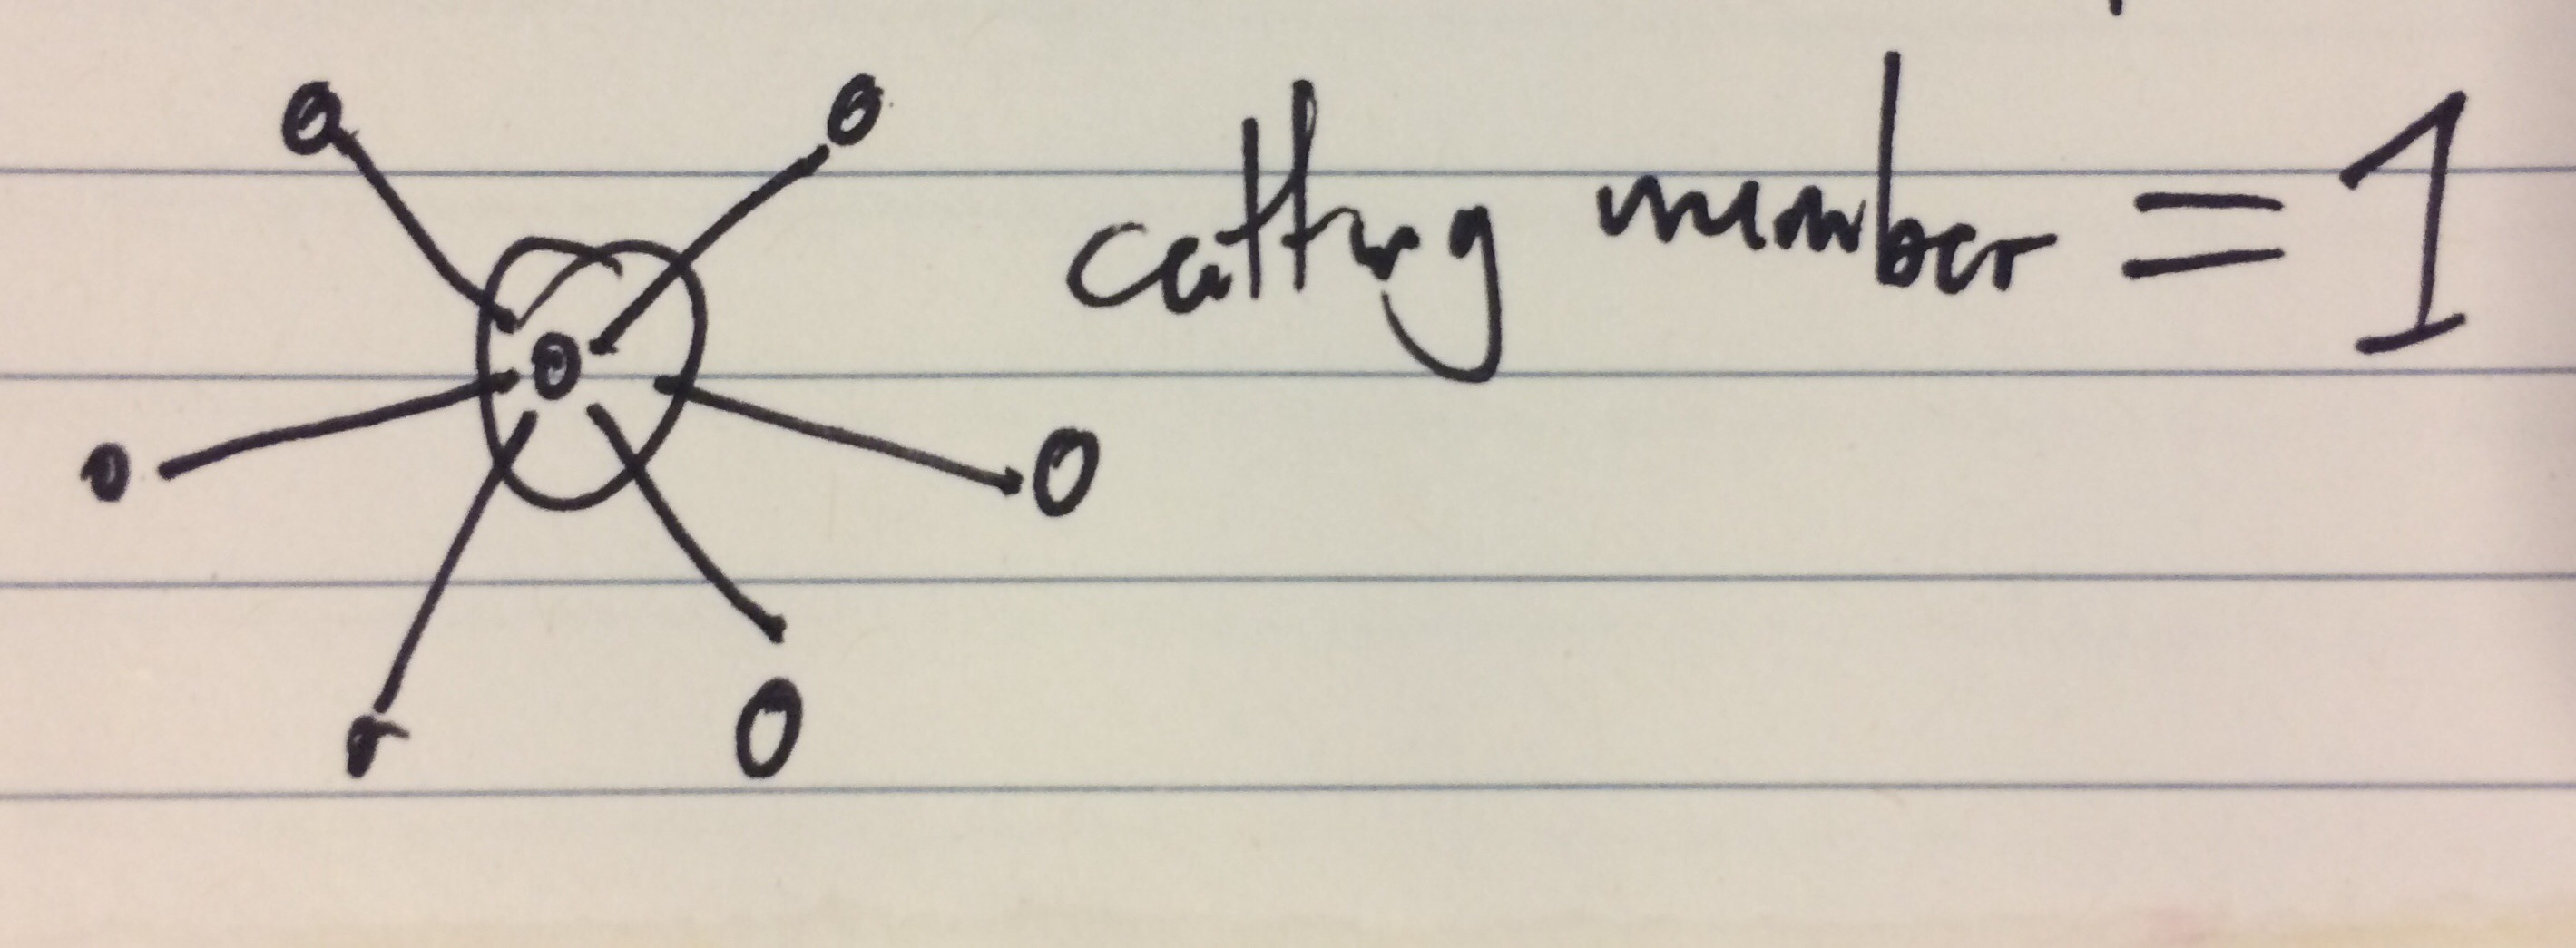
\includegraphics[scale=0.125]{lec2-3}

\subsubsection{Uber (Pathfinding)}

Pathfinding is a graph problem where $V$ represents all the intersections of a map and $E$ is all the roads. For a path $v_1, ... ,v_n$, the length is the number $m$, which is the sum of all the edge weights $\geq 0$, and for 2 connected vertices, we are trying to find the path of the least length. Dijsktra's Algorithm solves this problem.

\subsection{Morphism}

A morphism of graphs $G \mapsto G'$ consists of 2 functions:
\begin{itemize}
	\item{$\gamma_1 : V(G) \mapsto V(G')$}
	\item{$\gamma_2 : E(G) \mapsto E(G')$}
\end{itemize}

$\forall e$, if $e \in E(G)$ has endpoints $v_1, v_2$, this implies that $\gamma_2 (e)$ has endpoints $\gamma_1 (v_1), \gamma_1 (v_2)$.\\
\\
\begin{tcolorbox}
	Note: This definition is more general than the book.
\end{tcolorbox}

An isomorphism is a morphism such that $\gamma_1, \gamma_2$ are both bijective.
\\
\\
\underline{Example of a morphism:} (Note that $\simeq$ denotes a morphism)\\
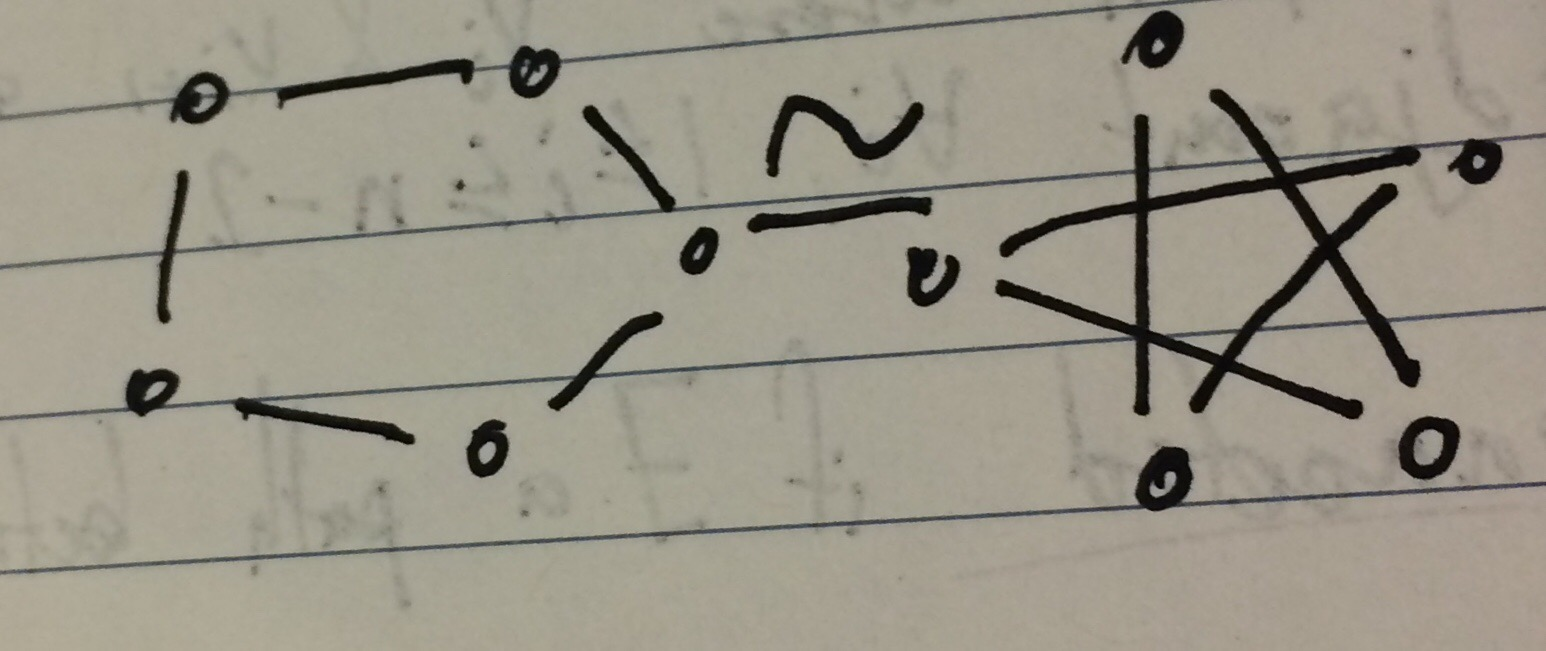
\includegraphics[scale=0.125]{lec2-4}

\newpage

\section{Tuesday, September 12, 2017}

\subsection{More Morphism}

\begin{tcolorbox}[title=Observation 1]
	if $G'$ is simple, there exists a morphism $G \mapsto G'$ and so $\gamma_1 : V(G) \mapsto V(G')$ such that if $e\in E(G)$ has endpoints $v_1, v_2$, then $\gamma_1 (v_1), \gamma_1 (v_2)$ are adjacent.
\end{tcolorbox}

A \textbf{subgraph} of $G$ is a subset $V' \subset V$, $E' \subset E$ such that $Id: (V', E') \mapsto G$ is a morphism.\\
\\
An \textbf{isomorphism} is when a morphism $G \mapsto G'$ is bijective (That there is a one to one relationship between $E \mapsto E'$ and $V \mapsto V'$)\\
\\
\underline{Exercise:} if $(\gamma_1, \gamma_2) : G \mapsto G'$ is an isomorphism, then $(\gamma_1^{-1}, \gamma_2^{-1}) : G' \mapsto G$\\
\\
\underline{Recall:} Bijective implies injective and surjective.

\begin{tcolorbox}[title=Definition: Complement of Simple Graphs]
	The complement of a simple graph $G$ is $\overset{\_\_\_}{G} = (\overset{\_\_\_}{V},\overset{\_\_\_}{E})$ where $V(\overset{\_\_\_}{G}) = V(G)$ and $\overset{\_\_\_}{E}$ does not have any edge in $E$, but if $v_1,v_2 \in V$ are not adjacent, then $v_1,v_2$ are adjacent in $\overset{\_\_\_}{G}$ for all $v_1,v_1 \in V$
\end{tcolorbox}

\underline{Example:}\\
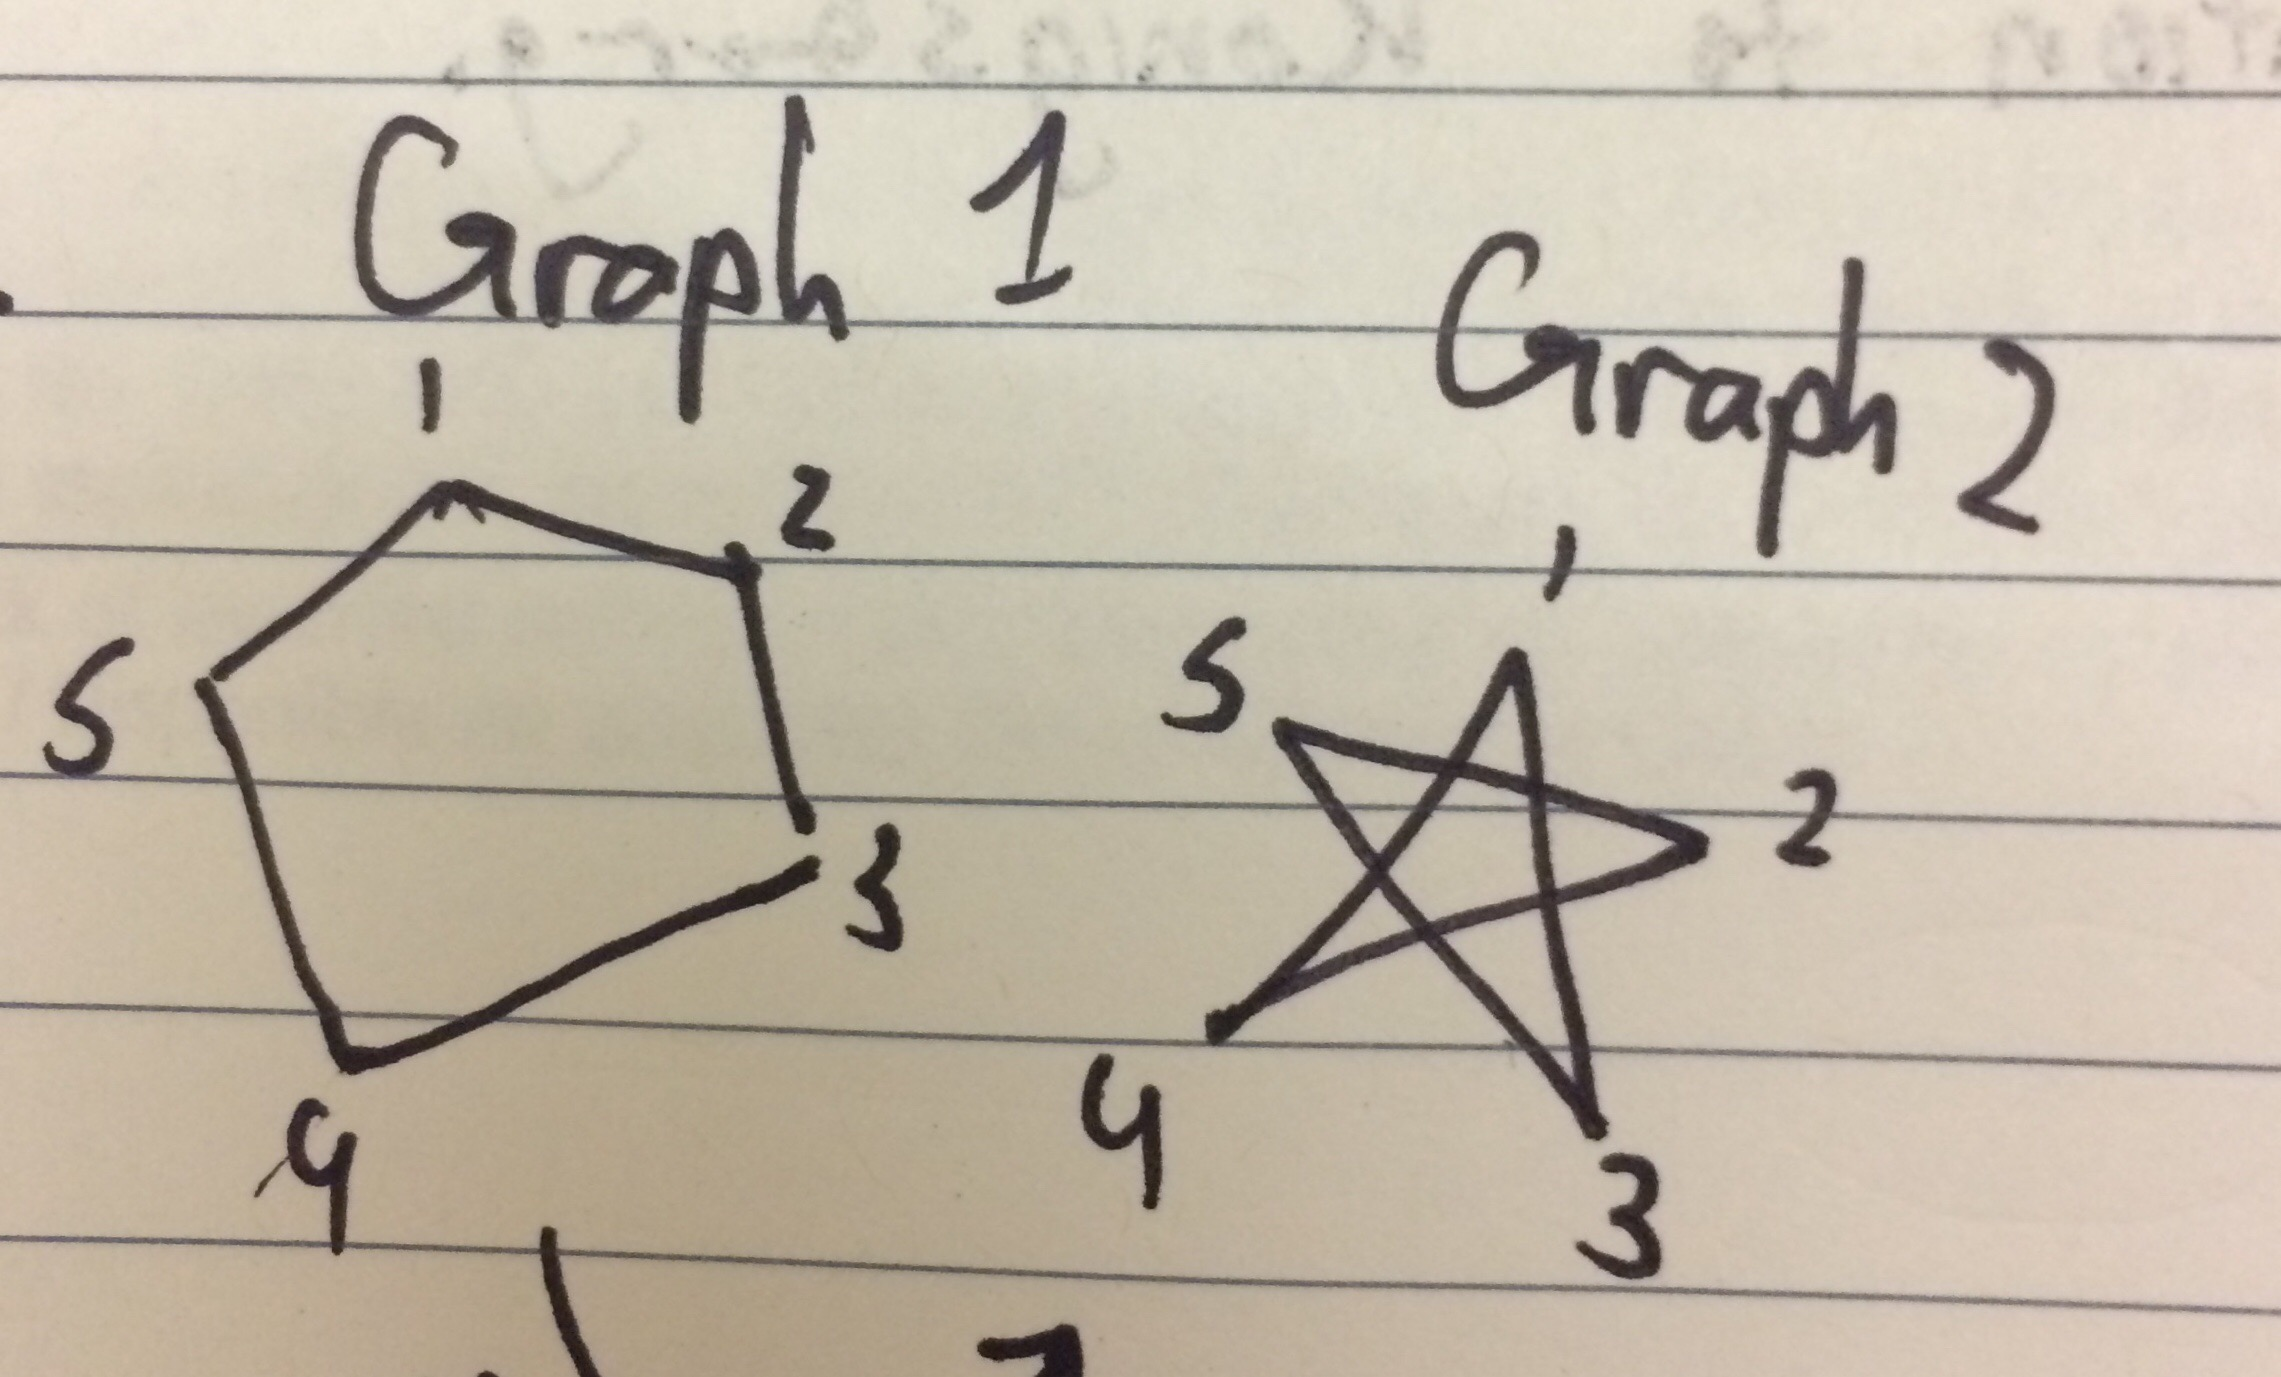
\includegraphics[scale=0.125]{lec3-1}\\
Graph 1 and Graph 2 are complements of each other.

We say a graph is \textbf{self-complementary} if a graph is isomorphic to its complement.

\subsection{Decomposing Graphs}

\begin{tcolorbox}[title=Definition: Union of Graphs]
	if $G_1, G_2$ are two graphs, assume $V(G_1), V(G_2) \subset V$ and $E(G_1), E(G_2) \subset E$. Then for a Graph $G_1 \cup G_2$
	\begin{itemize}
		\item{$V(G_1 \cup G_2) = V(G_1) \cup V(G_2)$}
		\item{$E(G_1 \cup G_2) = E(G_1) \cup E(G_2)$}
	\end{itemize}
\end{tcolorbox}

\underline{Example:}\\
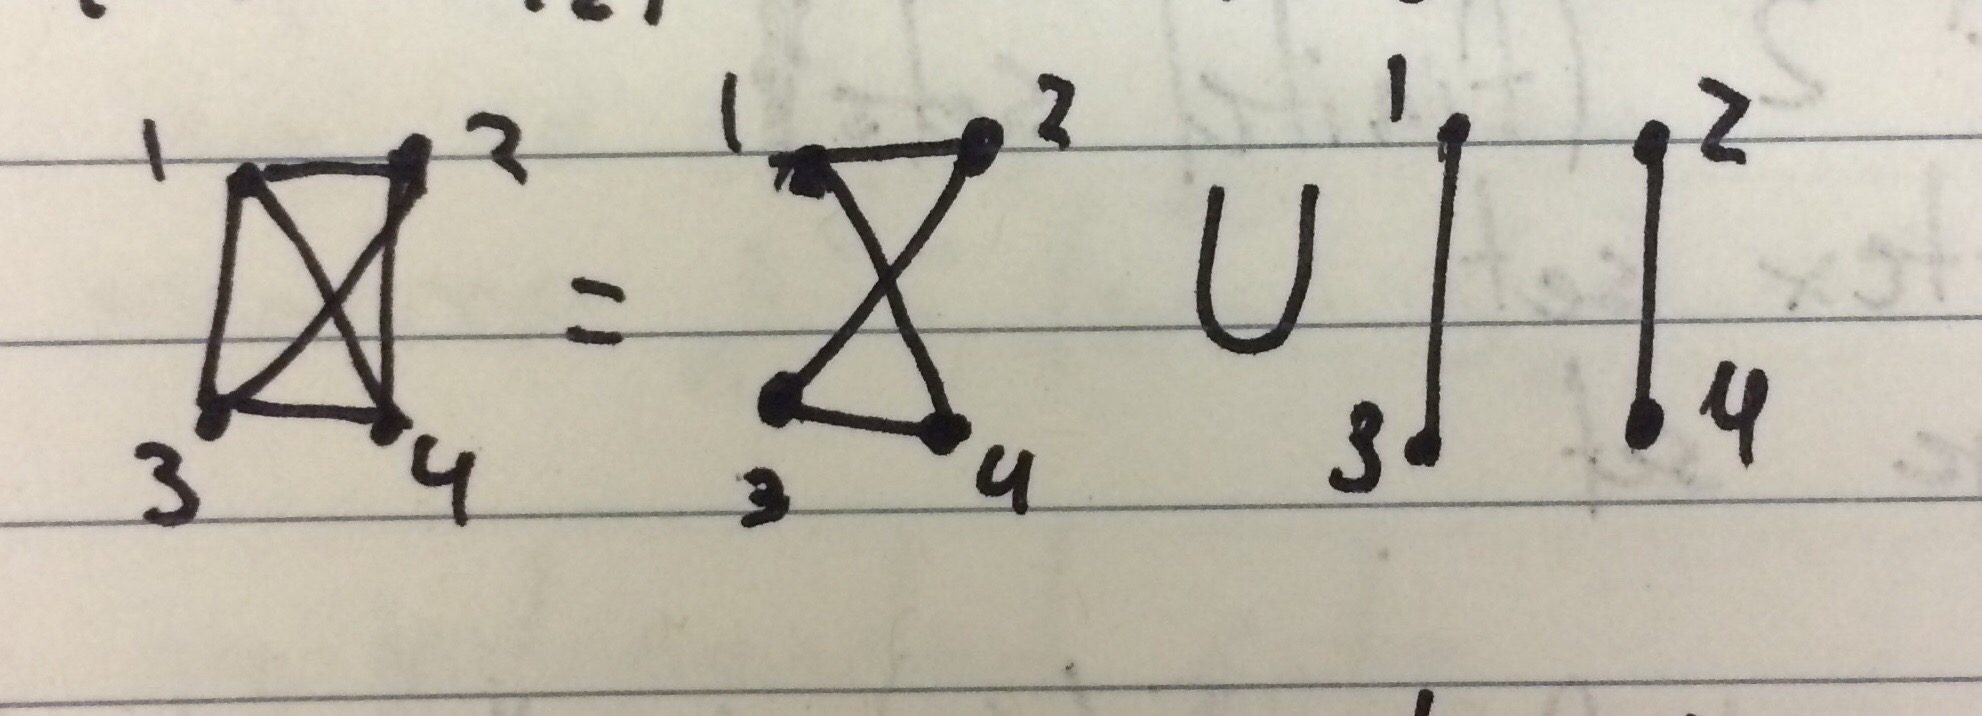
\includegraphics[scale=0.2]{lec3-2}\\

We say $G$ \textbf{decomposes} into $G_1$ and $G_2$ if the following:
\begin{itemize}
	\item{$G_1 \cup G_2 = G$}
	\item{if $\forall e \in E(G)$ there exists one $i$ such that $e\in E(G_i)$ (so if the edges between $G_1$ and $G_2$ don't overlap)}
\end{itemize}

\underline{Example:}\\
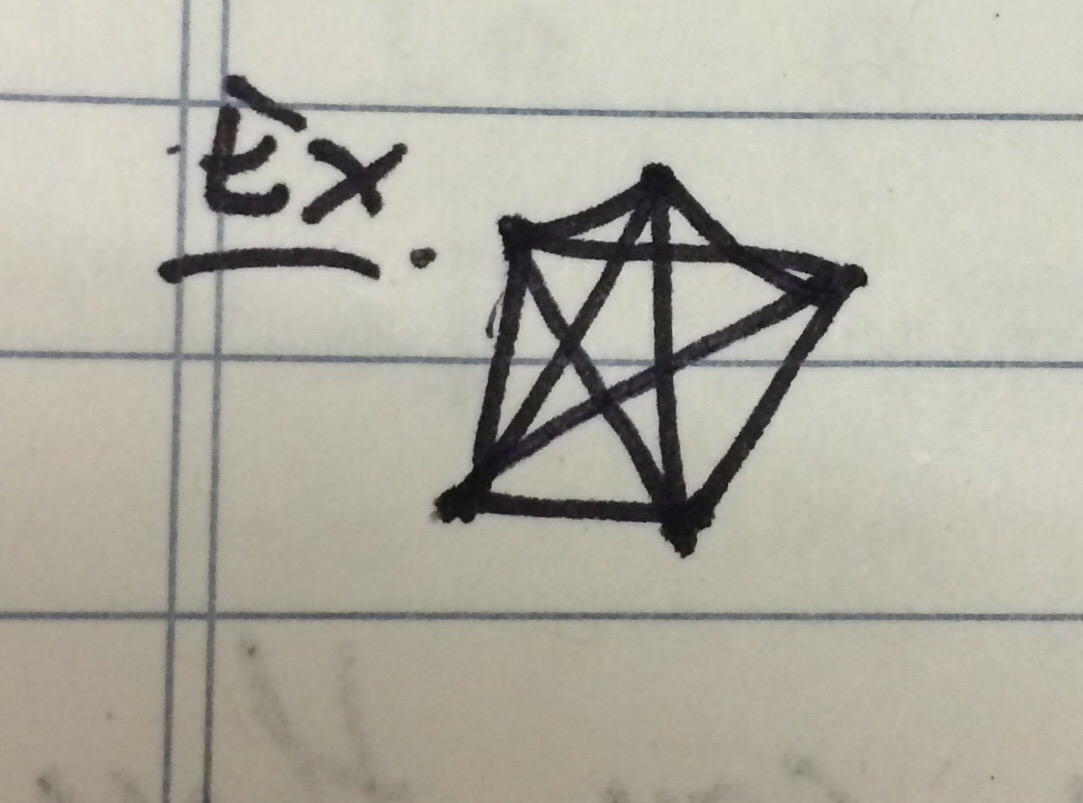
\includegraphics[scale=0.3]{lec3-3}\\
This is $k_5$, the complete simple graph of 5 vertices (complete meaning all vertices are adjacent)\\
\\
\underline{Example:}\\
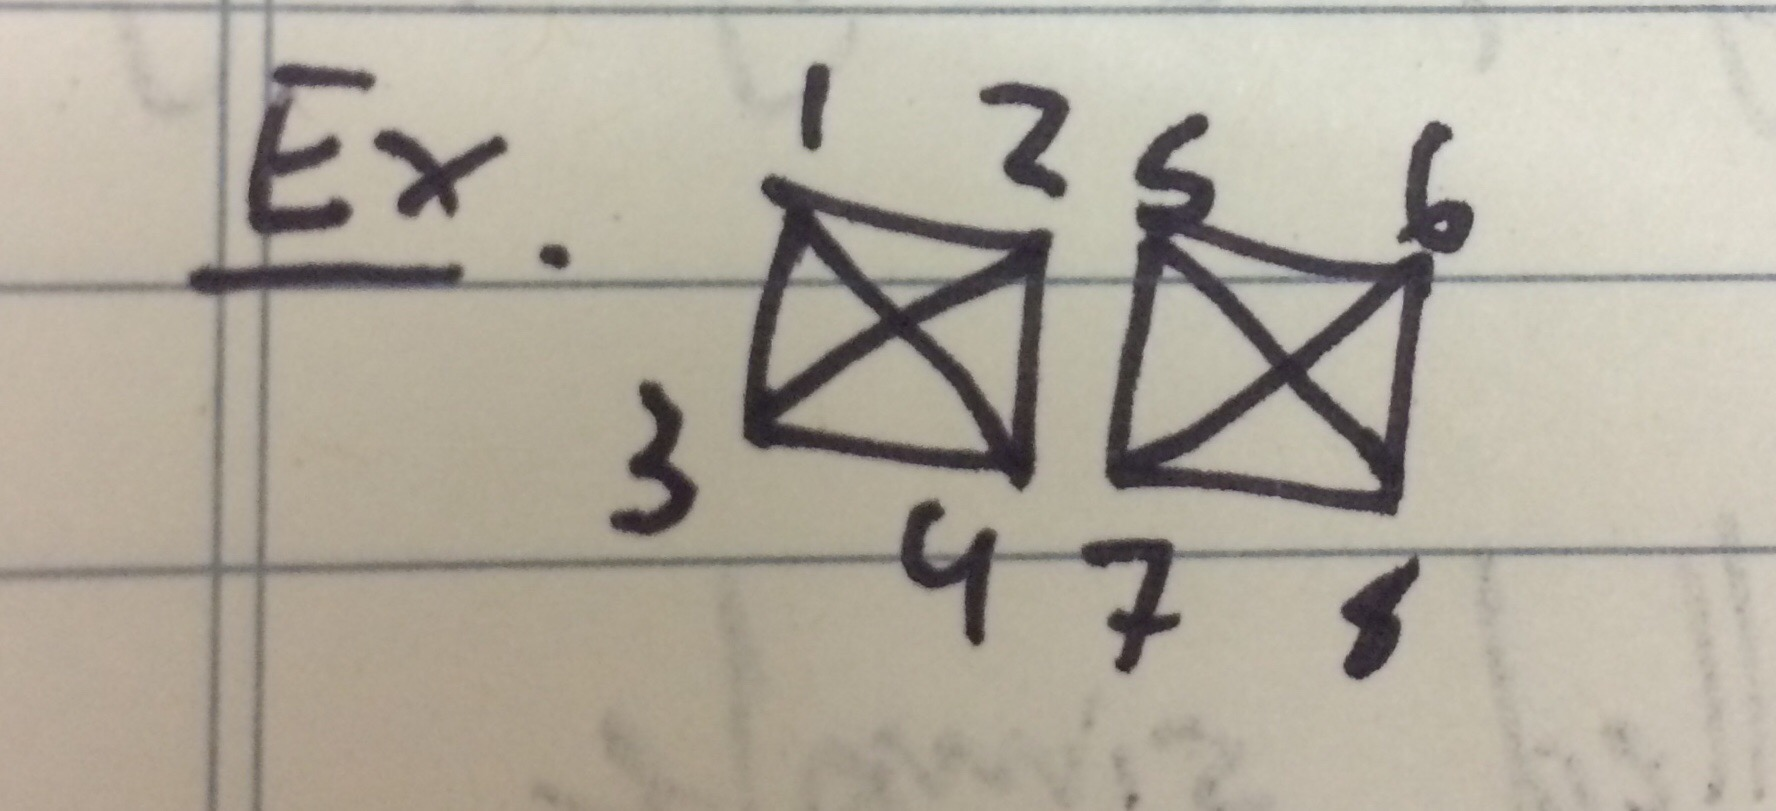
\includegraphics[scale=0.22]{lec3-4}\\
This is the disjoint union of 2 graphs. $G_1 $ SQUARE UNION $ G_2$ is the union of 2 graphs with $V(G_1) \cap V(G_2) = \emptyset$

\subsubsection{Connectivity of $G$}

\paragraph{Path} A path is a simple subgraph such that we can order vertices $v_1, ... ,v_{n-1}$ in such a way that exactly $v_i, v_{i+1}$ are adjacent $\forall i$

\paragraph{Cycle} A cycle is a subgraph that is simple and that we the vertices $v_1, ... ,v_{n}$, $v_1 = v_n$ such that exactly $v_i, v_{i+1}$ are adjacent $\forall i$ and that all edges are unique.\\
\\

\underline{Note:} the arrangement of vertices in a path is called a \textbf{walk}, the arrangement of vertices in a cycle is called a \textbf{trail}.\\
\\
we refer to an edge by $(u,v)$ where $u,v$ are the start and end vertices.

\newpage


\end{document}


























